\documentclass{mini}

\usepackage[utf8]{inputenc}
\usepackage{color}
\usepackage{xcolor}
\usepackage{tikz}
\usepackage{tikz-qtree}
\usepackage{caption}
\usepackage{subcaption}
\usepackage{multirow}

\usetikzlibrary{calc, shapes, backgrounds, arrows, positioning, calc}

\definecolor{mojkolor}{rgb}{0.99, 1, 0.99}
\newenvironment{dow}{\textbf{\textit{Dowód}}}{\begin{flushright} $\blacksquare$ \end{flushright}}
\newcommand{\argmin}{\arg\!\min}
\newcommand{\argmax}{\arg\!\max}

%------------------------------------------------------------------------------%
\title{Statystyczne metody regresji porządkowej}
\author{Marta Sommer}
\tytsupervisor{prof. nzw. dr hab.}
\supervisor{Przemysław Grzegorzewski}
\type{magisters}
\discipline{matematyka}
\monthyear{czerwiec 2015}
\date{\today}
\album{237503}
%------------------------------------------------------------------------------%

\begin{document}
\maketitle
\tableofcontents

\chapter*{Wstęp}

Regresja porządkowa (ang. \textit{ordinal regression}) jest jednym z działów uczenia maszynowego. Od problemu klasycznej regresji różni ją to, że zmienna odpowiedzi jest dyskretna, natomiast od problemu klasyfikacji to, że zmienna odpowiedzi ma pewien naturalny porządek. Regresja porządkowa zajmuje się zatem uczeniem i oceną jakości predyktora, który modeluje zmienną uporządkowaną i skończoną. Problem regresji porządkowej rozwija się dość szybko m.in. dlatego, że ma on bardzo wiele zastosowań, choćby w systemach rekomendacji, czy bardzo popularnych wyszukiwarkach internetowych. Prześledźmy to na konkretnym przykładzie. Wyobraźmy sobie sytuację, że chcielibyśmy określić, w jakim stopniu danemu człowiekowi spodoba się sprzedawany przez nas produkt. Mamy do dyspozycji zbiór treningowy składający się z wektora zmiennej objaśniającej $\textbf{x}=(x_1, \ldots, x_d)$, gdzie $x_i$ są różnymi cechami określającymi daną osobę (np. płeć, wiek, wykształcenie, ...). Cechy te -- podobnie jak w przypadku zwykłej regresji -- mogą być zarówno ciągłe, jak i dyskretne. Mamy również dostęp do zmiennej objaśnianej $\textbf{y}=(y_1, \ldots, y_r)$, będącej wektorem zero-jedynkowym, wskazującym która klasa została przypisana danemu rekordowi. W naszym przykładzie, zmienną odpowiedzi mogłyby być na przykład: \textit{zdecydowanie mi się nie podoba}, \textit{nie podoba mi się}, \textit{nie mam zdania}, \textit{podoba mi się}, \textit{zdecydowanie mi się podoba}. Widać wyraźnie, że są one uporządkowane.

Najprostszym podejściem do tego typu problemu byłoby zignorowanie kolejności zmiennej odpowiedzi i potraktowanie go, jak zwykłą klasyfikację. W takim przypadku tracimy jednak pewną informację, która prawdopodobnie mogłaby przyczynić się do poprawy naszego klasyfikatora. Idąc w drugą stronę, można potraktować nasz problem, jak zwykłą regresję, zamieniając zmienną odpowiedzi na pewną zmienną ciągłą i to ją modelując, a następnie z powrotem dyskretyzować. Pojawia się tu jednak problem, jak optymalnie zrobić taką transformację, uwzględniając chociażby fakt, że nasza odpowiedź niekoniecznie jest monotoniczna (tzn. np. różnica między \textit{nie podoba mi się} a \textit{nie mam zdania} wcale mnie musi być taka sama, jak między \textit{podoba mi się} a \textit{zdecydowanie mi się podoba}). 

Możemy wyróżnić dwa główne nurty w regresji porządkowej:
\begin{itemize}
	\item prognoza konkretnej obserwacji (nacisk kładziony jest tu na wyznaczenie konkretnego $\textbf{y}$ dla konkretnego $\textbf{x}$ np. czy potencjalnemu klientowi spodoba się dany produkt),
	\item uszeregowanie kilku obserwacji (celem nie jest poznanie estymacji konkretnej zmiennej odpowiedzi, ale takie uszeregowanie kilku rekordów, by te najbardziej preferowane znalazły się na samej górze, a te najmniej na samym dole np. w jakiej kolejności powinny wyświetlić się znalezione strony w wyszukiwarce). 
\end{itemize}

W mojej pracy zajmować się będę przede wszystkim pierwszym punktem, lecz nakreślę też kilka podejść dotyczących drugiego. 


\chapter{Opis teoretyczny dostępnych metod}


\section{Postawienie problemu i podstawowe oznaczenia}

Na wejściu dany mamy zbiór $\mathcal{D} = (\mathbf{x}^{(i)}, y^{(i)})_{i=1}^n$, składający się z $n$ par $(\mathbf{x}, y)$, gdzie:
\begin{itemize}
\item $\mathbf{x}^{(i)}$ jest $K$--wymiarowym wektorem cech (częstym założeniem będzie, że $\mathbf{x}^{(i)}\in \mathbb{R}^K$),  
\item $y^{(i)}$ jest liczbą symbolizującą kategorię, do której przyporządkowana została $i$--ta obserwacja, tzn. $y^{(i)}\in\mathcal{Y}$, gdzie $\mathcal{Y} = \lbrace 1,\ldots ,r \rbrace$ jest zbiorem uporządkowanym według pewnego porządku ,,$\prec$''. 
\end{itemize}
Naszym celem będzie stworzenie modelu, który pozwoli na wybranie najlepszej (nieznanej) kategorii $y_{\ast}\in\mathcal{Y}$ dla nowej obserwacji o zadanym wektorze cech $\mathbf{x}_{\ast}$. 

W tym rozdziale opracujemy kilka rozwiązań, które pozwolą nam się z tym problemem uporać.

\section{Model proporcjonalnych szans}

Najbardziej rozpowszechnionym sposobem modelowania regresji porządkowej jest model proporcjonalnych szans. Jest to jedna z metod uogólnionych modeli liniowych, bardzo silnie opierająca się na regresji logistycznej. Interesują nas prawdopodobieństwa: 
$$
\Pi_j(\mathbf{x}):=\mathbb{P}(y_=j\hspace{1mm}|\hspace{1mm}\mathbf{x}),\quad \textrm{dla}\hspace{3mm} j=1,\ldots,r.
$$
Idea polega nie na bezpośrednim modelowaniu prawdopodobieństw $\Pi_j(\mathbf{x})$, lecz na wcześniejszym modelowaniu tzw. prawdopodobieństw skumulowanych:
$$
\mathbb{P}(y\leq j \hspace{1mm}|\hspace{1mm} \mathbf{x})=\Pi_1(\mathbf{x})+\ldots+\Pi_j(\mathbf{x}),\quad \textrm{dla}\hspace{3mm} j=1,\ldots,r-1.
$$
Następnie rozważa się poniższy model logitowy:
$$
\log\dfrac{\mathbb{P}(y\leq j \hspace{1mm}|\hspace{1mm} \mathbf{x})}{1 - \mathbb{P}(Y\leq j \hspace{1mm}|\hspace{1mm} \mathbf{x})} = \alpha_j+\mathbf{\beta}^T\mathbf{x},\quad \textrm{dla}\hspace{3mm} j=1,\ldots,r-1,
$$
gdzie $\alpha_j\in \mathbb{R}$ i $\mathbf{\beta}\in \mathbb{R}^K$ są parametrami modelu. Należy zauważyć, że parametr $\beta$ jest stały dla każdego $j=1, \ldots, r-1$.

Współczynniki modelu -- jak w przypadku regresji logistycznej -- wyliczamy metodą Raphsona-Newtona, a skumulowane prawdopodobieństwa -- po prostym przeliczeniu -- dostaniemy ze~wzoru:
$$
\mathbb{P}(y\leq j \hspace{1mm}|\hspace{1mm} \mathbf{x})=\dfrac{e^{\alpha_j+\mathbf{\beta}^T\mathbf{x}}}{1+e^{\alpha_j+\mathbf{\beta}^T\mathbf{x}}},\quad \textrm{dla}\hspace{3mm} j=1,\ldots,r-1.
$$ 
Szukane prawdopodobieństwa $\Pi_j(\mathbf{x})$ otrzymamy w poniższy sposób:
\begin{eqnarray*}
\Pi_1(\mathbf{x}) &=& \mathbb{P}(Y\leq 1 \hspace{1mm}|\hspace{1mm}\mathbf{x}),\\
&\vdots&\\
\Pi_i(\mathbf{x}) &=& \mathbb{P}(Y\leq i \hspace{1mm}|\hspace{1mm} \mathbf{x}) - \mathbb{P}(Y\leq i-1 \hspace{1mm}|\hspace{1mm} \mathbf{x}),\\
&\vdots&\\
\Pi_r(\mathbf{x}) &=& 1 - \mathbb{P}(Y\leq r-1 \hspace{1mm}|\hspace{1mm} \mathbf{x}).
\end{eqnarray*}

Dla nowej obserwacji $\mathbf{x}_{\ast}$ wybieramy oczywiście klasę $y_{\ast}$, która maksymalizuje prawdopodobieństwa $\Pi_j(\mathbf{x}_{\ast})$.

\section{Wektory maszyn podpierających (SVM)}

Wektory maszyn podpierających (ang. \textit{Support Vector Machine}) to bardzo znana i powszechnie stosowana metoda klasyfikacji. W dużym uproszczeniu, polega ona na konstrukcji dwóch równoległych i maksymalnie oddalonych od siebie hiperpłaszczyzn w taki sposób, by minimalizować kwadrat odległości między nimi. By móc obsługiwać przypadki, w których brak liniowej separowalności, wprowadza się dodatkowo karę za nieidealne rozdzielenie klas. W przypadku dwuklasowym budowa modelu sprowadza się do rozwiązania następującego problemu optymalizacyjnego:
$$
\min\left\lbrace\dfrac{1}{2}||\textbf{w}||^2+C\sum_{i=1}^{n}\xi_i\right\rbrace
$$
przy ograniczeniach:
$$
\begin{cases}
\mathbf{x}^{(i)^T}\textbf{w}+b &\geq 1-\xi_i\\
\mathbf{x}^{(i)^T}\textbf{w}+b &\leq -1+\xi_i,
\end{cases}
$$    
gdzie $\mathbf{w}\in\mathbb{R}^K$, $b\in\mathbb{R}$, $C\in\mathbb{R}$ i $\xi_i\geq 0$ są parametrami modelu.

Tak to wyglądało w przypadku dwuklasowej klasyfikacji. Przyjrzyjmy się teraz, jak w łatwy sposób można zaadaptować powyższą metodę do rozważanej przez nas regresji porządkowej.

\begin{figure}[h]
\begin{center}
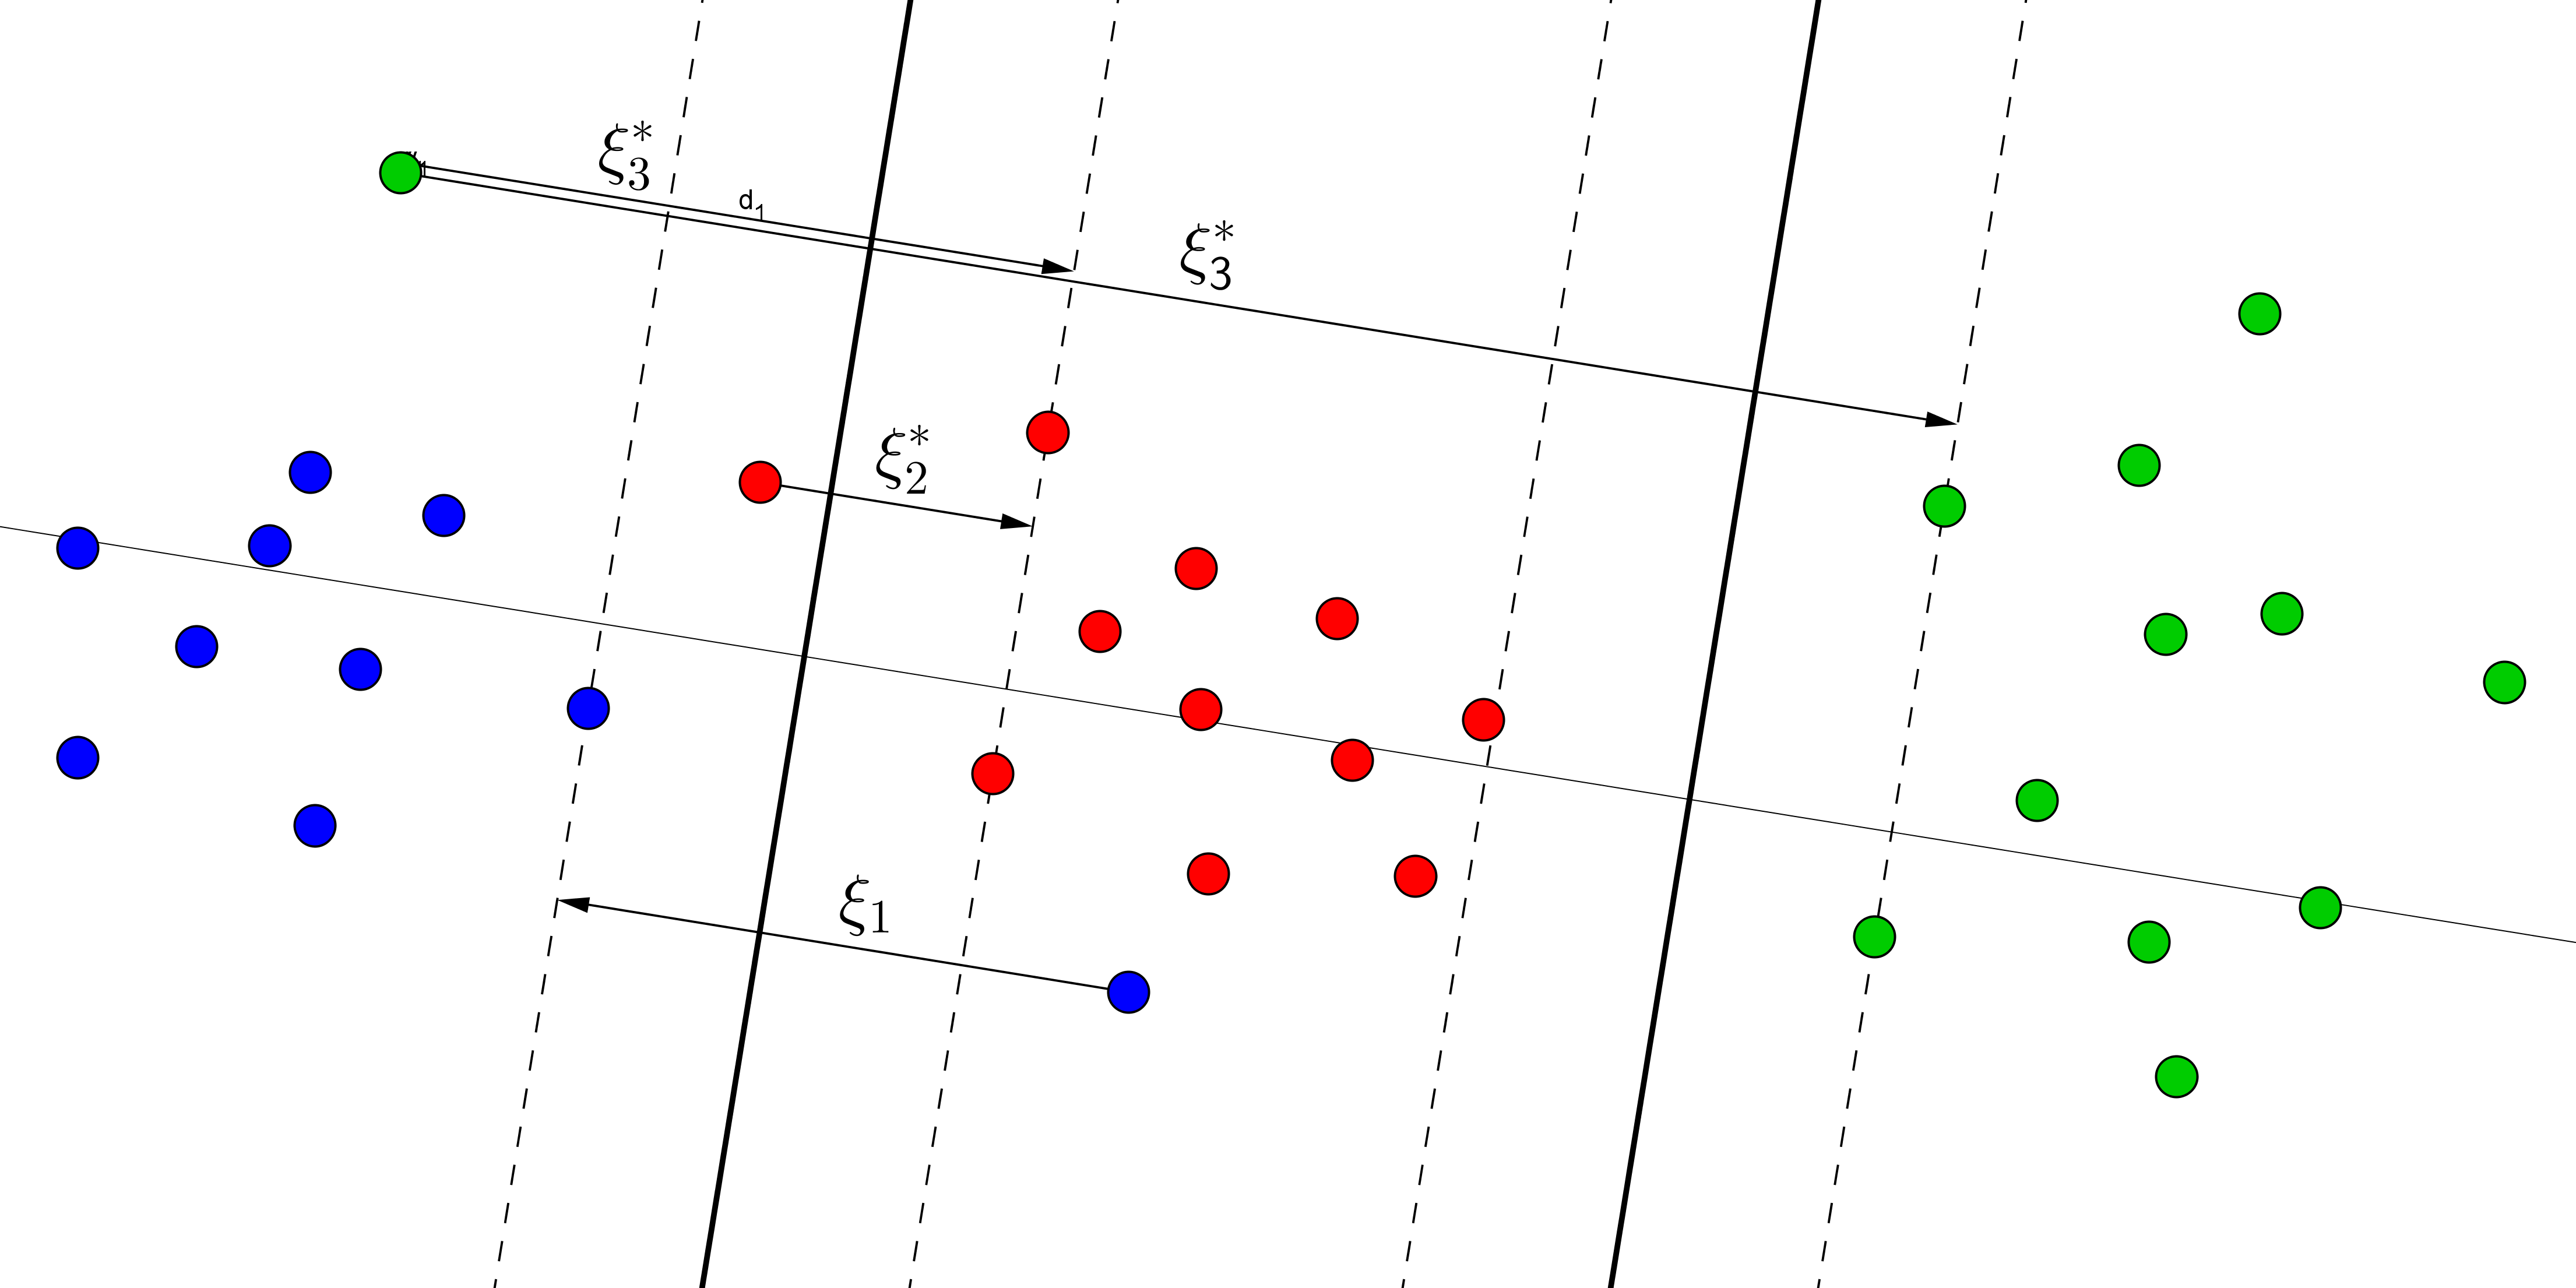
\includegraphics[width=\textwidth]{svm3.png}
\end{center}
\caption{Przykładowa klasyfikacja metodą SVM.}
\end{figure}

Tym razem optymalizować będziemy następujące wyrażenie:
$$
\min_{\textbf{w}, b_k}\left\lbrace \dfrac{1}{2}||\textbf{w}||^2+C\sum_{j=1}^{r-1}\left( \sum_{k=1}^{j}\sum_{i=1}^{n_k}\xi_{ki}^j+\sum_{k=j+1}^{r}\sum_{i=1}^{n_k}\xi_{ki}^{*j}\right)\right\rbrace
$$
przy ograniczeniach:
$$
\begin{cases}
\textbf{w}x^{(i)}_k-b_j&\leq -1 +\xi^j_{ki}, \hspace{6mm} \textrm{dla}\hspace{3mm} k=1,\ldots,j \hspace{3mm}\textrm{oraz}\hspace{3mm} i=1,\ldots,n_k \\
\textbf{w}x^{(i)}_k-b_j&\geq +1 -\xi^{*j}_{ki}, \hspace{6mm} \textrm{dla}\hspace{3mm} k=j+1,\ldots,r \hspace{3mm}\textrm{oraz}\hspace{3mm} i=1,\ldots,n_k 
\end{cases}
$$

Przyjrzyjmy się, czym różni się nasz nowy problem od problemu optymalizacyjnego w standardowej klasyfikacji. Przede wszystkim -- podobnie jak w modelu proporcjonalnych szans -- mamy tu do czynienia z $(r-1)$--hiperpłaszczyznami, rzutowanymi na jeden, wspólny dla wszystkich obserwacji, kierunek $\mathbf{w}$. Przy wyznaczaniu kolejnych hiperpłaszczyzn, bierzemy pod uwagę wszystkie klasy. Kary naliczane są więc w następujący sposób. Dla progu $b_j$, wartości funkcji $\textbf{w}x^{(i)}_k$ dla obserwacji z niższych klas, powinny być niższe niż dolna granica $b_j-1$. Jeśli tak nie jest, wtedy jako błąd próbki $\xi^j_{ki}$ dla progu $b_j$ uznaje się $\xi^j_{ki} = \textbf{w}x^{(i)}_k-(b_j - 1)$. Analogicznie, dla obserwacji z wyższych klas, otrzymujemy błędy $\xi^{*j}_{ki}$.

Budowa modelu i tym razem sprowadza się więc do problemu optymalizacyjnego.

\section{Sieci neuronowe}
 
Sieci neuronowe to bardzo proste i szeroko stosowane narzędzie zarówno w problemach regresji, jak i klasyfikacji. Znalazło ono również swoje zastosowanie w regresji porządkowej (por. \cite{nna}). 

Standardowo, na wejściu otrzymujemy zbiór uczący w postaci $n$ par $(\textbf{x},y)$, gdzie $\textbf{x} = (x_1, \ldots, x_K)^T$ jest wektorem cech, a $y$ numerem klasy. Tym razem jednak, dodatkowo modyfikujemy zmienną odpowiedzi w taki sposób, by zamiast liczby rzeczywistej otrzymać zero-jedynkowy wektor odpowiedzi $\textbf{y} = (y_1, \ldots, y_r)^T$ reprezentujący klasę, do której należy dana obserwacja, tzn. $y_i = \mathbb{I}\lbrace y =i \rbrace$.

W przeciwieństwie do zwykłej klasyfikacji, nasza sieć neuronowa będzie zakładać porządek zmiennej odpowiedzi. W jaki sposób? Mianowicie, jako wektor wyjściowy, zamiast wektora $\textbf{y} = (0, 0, \ldots, 1, \ldots, 0)^T$, mającego jedynkę na $i$--tym miejscu, jeśli obserwacja należała do $i$--tej klasy, rozważać będziemy wektor $\textbf{y} = (1, 1, \ldots, 1, \ldots, 0)^T$, mający jedynki na miejscach od pierwszego do $i$--tego.

Otrzymujemy w ten sposób sieć neuronową o $K$ neuronach w warstwie wejściowej, z których każdy reprezentuje inną cechę z wektora $\textbf{x}$, jednej (bądź więcej) warstwie ukrytej o $m$ neuronach i warstwie wyjściowej zawierającej $r$ neuronów, które reprezentują odpowiedź $\textbf{y}$ w formie opisanej powyżej. Za funkcję przejścia przyjmiemy funkcję sigmoidalną $f(x) = \frac{1}{1+e^{-x}}$, dobrze reprezentującą przynależność do danej klasy jako prawdopodobieństwo. Może się zdarzyć, że wyjściowy wektor nie będzie ciągiem malejącym (co trochę przeczy intuicji), jednak nie jest to konieczne do robienia predykcji. 

\begin{figure}[h]
\begin{center}

	\def\layersep{6cm}

\begin{tikzpicture}[shorten >=1pt, ->, draw=black!50, node distance=\layersep]
    \tikzstyle{neuron}=[circle, fill=black!25, minimum size=17pt, inner sep=0pt]
    \tikzstyle{input neuron}=[neuron, fill=green!50];
    \tikzstyle{output neuron}=[neuron, fill=red!50];
    \tikzstyle{hidden neuron}=[neuron, fill=blue!50];
    \tikzstyle{annot} = [text width=5em, text centered]

    \foreach \name / \y in {1/1,K/3}
        \node[input neuron] (I-\y) at (0,-3*\y) {$\text{wyjscie}^{(0)}_\name$};
    \node[draw=none, scale=4, text height=0.333cm] (I-2) at (0,-3*2) {$\vdots$};

	\foreach \name / \y in {1/1, 2/2, m/4}
        \path[yshift=1.4cm]
            node[hidden neuron] (H-\y) at (\layersep,-3*\y cm) {$\text{wyjscie}^{(1)}_{\name}$};
    \path[yshift=1.4cm]
            node[draw=none, scale=4, text height=0.333cm] (H-3) at (\layersep,-3*3 cm) {$\vdots$};

	\foreach \name / \y in {1/1, r/3}
        \path[yshift=0cm]
            node[output neuron] (O-\y) at (2*\layersep,-3*\y cm) {$\text{wyjscie}^{(2)}_{\name}$};
    \path[yshift=0cm]
            node[draw=none, scale=4, text height=0.333cm] (O-2) at (2*\layersep,-3*2 cm) {$\vdots$};

	\foreach \source / \sname in {1/1,3/K}
        \foreach \dest / \dname in {1/1,2/2,4/m}
            \path (I-\source) edge node[pos=0.25, sloped, fill=mojkolor, opacity=0.9, text opacity=1]{$w_{\sname\rightarrow\dname}^{(1)}$} (H-\dest);
    \foreach \source / \sname in {1/1,2/2,4/m}
    	\foreach \dest / \dname in {1/1,3/r}
        \path (H-\source) edge node[pos=0.75, sloped, fill=mojkolor, opacity=0.9, text opacity=1]{$w_{\sname\rightarrow\dname}^{(2)}$} (O-\dest);
        
    \node[annot,above of=H-1, node distance=1.5cm] (hl) {Warstwa ukryta};
    \node[annot,left of=hl] {Warstwa wejściowa};
    \node[annot,right of=hl] {Warstwa wyjściowa};

\end{tikzpicture}
\end{center}
\caption{Przykładowa sieć neuronowa.}
\end{figure}

Uczenie sieci neuronowej będzie się odbywało algorytmem propagacji wstecznej z kwadratową funkcją straty (można też użyć jakiejś innej np. entropii). Algorytm wygląda następująco:
\begin{enumerate}
\item Wybieramy małe wagi początkowe oraz niewielki współczynnik $\eta>0$.
\item Losujemy parę $(\textbf{x},\textbf{y})$ ze zbioru uczącego.
\item Przebiegamy sieć w przód.
\item Przebiegamy sieć w tył (licząc błąd dla każdego neuronu).
\item Zmieniamy wagi.
\item Dopóki nie osiągniemy zadowalająco niskiego błędu, wracamy do punktu $2)$.
\end{enumerate} 

\underline{Ad. $3)$} 

Dla każdego neuronu obliczamy wartość wejściową ze wzoru:
$$
wejscie_j^{(i)} = \sum_{k:\hspace{2mm}\exists\hspace{2mm} w^{(i)}_{k\rightarrow j}} \left( w^{(i)}_{k\rightarrow j}\cdot wyjscie_k^{(i-1)} \right),
$$
gdzie $wyjscie_i^{(0)} = x_i$. A następnie wyjściową:
$$
wyjscie_j^{(i)} = f\left(wyjscie_j^{(i)}\right). 
$$

\underline{Ad. $4)$}

Dla warstwy wyjściowej błąd ma postać:
$$
\delta_j = -2\cdot wyjscie_j^2\cdot \left( 1- wyjscie_j \right)^2\cdot(y_j - wyjscie_j),
$$
zaś dla warstw ukrytych:
$$
\delta_j^{(i)} =  wyjscie_j^{(i)}\cdot \left( 1- wyjscie_j^{(i)} \right) \cdot \sum_{k:\hspace{2mm}\exists\hspace{2mm} w^{(i+1)}_{j\rightarrow k}} \left( w^{(i+1)}_{j\rightarrow k}\cdot \delta_k^{(i-1)} \right).
$$

\underline{Ad. $5)$}

Modyfikacja wag przebiega następująco:
$$
w_{k\rightarrow j}^{(i)^{(new)}} = w_{k\rightarrow j}^{(i)^{(old)}} - \eta\cdot\delta_j^{(i)}\cdot wyjscie^{(i-1)}_k.
$$

Predykcja opiera się już tylko na przejściu algorytmu w przód z nowymi obserwacjami wejściowymi $\textbf{x}_{\ast}$ i ustaleniu progu (najczęściej równego $0,5$), klasyfikującego neuron wyjściowy jako jedynkę. Skanujemy wektor wyjściowy zaczynając od $y_1$ i kończymy, gdy pierwszy raz natkniemy się na $0$. Przypisujemy obserwacji taką klasę, jaką długość miał znaleziony przez nas ciąg jedynek.

\section{Metoda zaproponowana przez E. Franka i M. Halla}

Podejście Franka i Halla (por. \cite{fh}) do zagadnienia regresji porządkowej jest nieco inne, niż przedstawione do tej pory metody. Opiera się bowiem nie na stworzeniu nowego modelu, ale na odpowiednim przedefiniowaniu zbioru danych, a następnie na sprowadzeniu zadania do problemu zwykłej klasyfikacji z dwoma klasami. Przekształcamy zatem $r$--klasowy model regresji porządkowej do $(r-1)$ dwuklasowych problemów klasyfikacji. 

Algorytm do budowy modelu wygląda następująco:

\begin{enumerate}
\item Modyfikujemy zbiór uczący (otrzymując $r-1$ nowych zbiorów uczących).
\item Dla każdego nowo uzyskanego zbioru danych dopasowujemy zwykły model klasyfikacyjny (np. drzewo) taki, który zwraca prawdopodobieństwa przynależności do klas.
\item Robimy predykcję dla nowej obserwacji. 
\end{enumerate}

\begin{figure}[h]
\begin{center}
	\begin{tikzpicture}
		\node(gora) {\begin{tabular}{c|c}
					$\mathbf{x}$ & $y$ \\
					[1ex] \hline \\ [-1.5ex] 
					$x_1^{(1)}$ $\ldots$ $x_K^{(1)}$ & $y_1$ \\
					[1ex] $x_1^{(2)}$ $\ldots$ $x_K^{(2)}$ & $y_r$ \\
					[1ex] \vdots & $\vdots$ \\
					[1ex] $x_1^{(n)}$ $\ldots$ $x_K^{(n)}$ & $y_2$\\
				\end{tabular}};
		\node [below= 4cm of gora] (srodek) {$\ldots$};
		\node [right= 3cm of srodek] (prawo) {\begin{tabular}{c|c}
					$\mathbf{x}$ & $y^{(r-1)}$ \\
					[1ex] \hline \\ [-1.5ex] 
					$x_1^{(1)}$ $\ldots$ $x_K^{(1)}$ & $0$ \\
					[1ex] $x_1^{(2)}$ $\ldots$ $x_K^{(2)}$ & $1$ \\
					[1ex] \vdots & $\vdots$ \\
					[1ex] $x_1^{(n)}$ $\ldots$ $x_K^{(n)}$ & $0$\\
				\end{tabular}};
		\node [left= 3cm of srodek] (lewo) {\begin{tabular}{c|c}
					$\mathbf{x}$ & $y^{(1)}$ \\
					[1ex] \hline \\ [-1.5ex] 
					$x_1^{(1)}$ $\ldots$ $x_K^{(1)}$ & $0$ \\
					[1ex] $x_1^{(2)}$ $\ldots$ $x_K^{(2)}$ & $1$ \\
					[1ex] \vdots & $\vdots$ \\
					[1ex] $x_1^{(n)}$ $\ldots$ $x_K^{(n)}$ & $1$\\
				\end{tabular}};
		\path[draw, -latex',thick] (gora) -- (lewo);
		\path[draw, -latex',thick] (gora) -- (prawo);
	\end{tikzpicture}
\end{center}
\caption{Modyfikacja przykładowego zbioru uczącego.}
\end{figure}

\underline{Ad. $1)$}

Chcemy otrzymać $r-1$ nowych zbiorów o zero-jedynkowej zmiennej odpowiedzi. W jaki sposób to zrobić?
Macierz atrybutów pozostaje bez zmian, zmienia się jedynie wektor zmiennej odpowiedzi według zasady:
\begin{eqnarray*}
y_i^{(1)} &=& \mathbb{I}\lbrace y_i>1 \rbrace\\
&\vdots& \\
y_i^{(r-1)} &=& \mathbb{I}\lbrace y_i>r-1 \rbrace\\
\end{eqnarray*}

\underline{Ad. $3)$}

Dla nowego wektora atrybutów $\textbf{x}$ robimy predykcję na $r-1$ modelach uzyskanych w punkcie $2)$. Zwracamy jednak nie predykcję klasy, ale prawdopodobieństwo przynależności do klasy pierwszej. Uzyskujemy w ten sposób $r-1$ następuących prawdopodobieństw:
\begin{eqnarray*}
\mathbb{P}(y &>& 1)\\
&\vdots& \\
\mathbb{P}(y &>& r-1).\\
\end{eqnarray*}

Nas natomiast interesują prawdopodobieństwa:
\begin{eqnarray*}
\mathbb{P}(y &=& 1)\\
&\vdots& \\
\mathbb{P}(y &=& r-1).\\
\end{eqnarray*}

Łatwo otrzymamy korzystając z następującego wzoru łańcuchowego:
\begin{eqnarray*}
\mathbb{P}(y = 1) &=& 1 - \mathbb{P}(y > 1)\\
&\vdots& \\
\mathbb{P}(y = i) &=& \mathbb{P}(y > i-1) - \mathbb{P}(y > i) \qquad \text{dla}\hspace{5mm} i=2, \ldots, r-1\\
&\vdots& \\
\mathbb{P}(y = r) &=& \mathbb{P}(y > r-1).\\
\end{eqnarray*}

Ostatecznie, nowej obserwacji przypisujemy klasę, której prawdopodobieństwo $\mathbb{P}(y=i)$ było największe.

\section{Procesy gaussowskie}

Kolejną metodą modelowania problemu regresji porządkowej jest użycie procesu gaussowskiego. Jest to metoda popularna szczególne przy zwykłej regresji, znalazła ona jednak również zastosowanie w klasyfikacji zarówno jedno, jak i wieloetykietowej. Chu i Ghahramani w pracy \cite{reg} pokazują, jak rozszerzyć ją na regresję porządkową. 

Pomysł modelowania regresji porządkowej polega na wprowadzeniu tzw. zmiennej ukrytej, będącej niejako krokiem pośrednim w modelowaniu zmiennej odpowiedzi. W celu wyrobienia sobie intuicji, przeanalizujmy całe rozumowanie nieco od tyłu, zaczynając od predykcji. Podstawowym założeniem \textit{a priori} tej metody jest to, że zmienna ukryta $f$ jest procesem gaussowskim tzn., że jej rozkłady skończenie wymiarowe są normalne. Pełną charakteryzację takiego procesu tworzą dwie informacje -- średnia (standardowo przyjmuje się $0$) oraz macierz kowariancji $\mathbf{\Sigma}$. Dla celów tej pracy przyjmiemy, że elementy macierzy kowariancji definiowane są w następujący sposób:
$$
\mathbf{\Sigma}_{ij} = \mathbf{\Sigma}(x_i, x_j) = \exp \left\lbrace -\frac{\kappa}{2}\sum_{\xi=1}^K (x_i^{\xi} - x_j^{\xi})^2\right\rbrace,
$$
gdzie $\kappa>0$, a $x_i^{\xi}$ oznacza $\xi$-ty element wektora $\mathbf{x}_i$. Zatem $\mathbf{f} | \mathbf{X} \sim \mathcal{N}(0, \mathbf{\Sigma})$, czyli:
\begin{equation}\label{apriori}
\mathbb{P}(\mathbf{f} | \mathbf{X}) = \frac{1}{(2\Pi)^{\frac{n}{2}}|\mathbf{\Sigma}|^{\frac{1}{2}}}\exp\left\lbrace -\frac{1}{2}\mathbf{f}^T\mathbf{\Sigma}^{-1}\mathbf{f} \right\rbrace,
\end{equation}
gdzie $\mathbf{f} = [f(\mathbf{x}_1), \ldots, f(\mathbf{x}_n)]^T$ to wektor zawierający realizację zmiennej ukrytej, odpowiadający kolejnym obserwacjom ze zbioru uczącego.

Wyobraźmy sobie teraz, że dopasowaliśmy model i znamy wszystkie niezbędne parametry. W uproszczony sposób predykcja wygląda następująco: 
\begin{enumerate}
\item na wejściu otrzymujemy nową obserwację o danym wektorze cech $\textbf{x}_{\ast}$,
\item w pewien sposób wyliczamy dla niej liczbę rzeczywistą $f(\mathbf{x}_{\ast})$,
\item  za pomocą przekształcenia prostej rzeczywistej na $r$ podzbiorów, wyznaczamy najlepszy $y_{\ast}$.
\end{enumerate}

A teraz prześledźmy wszystko krok po kroku. Interesuje nas wyznaczenie $y_{\ast}$, dla którego prawdopodobieństwo $\mathbb{P}(y_{\ast} | \textbf{X}, \textbf{y}, x_{\ast})$ jest największe. Przy pomocy zmiennej ukrytej rozpiszmy je w następujący sposób:
\begin{equation}\label{calka1}
\mathbb{P}(y_{\ast} | \textbf{X}, \textbf{y}, \mathbf{x}_{\ast}) = \int \mathbb{P}(y_{\ast} | f(\mathbf{x}_{\ast}))\mathbb{P}(f(\mathbf{x}_{\ast}) | \textbf{X}, \textbf{y}) df(\mathbf{x}_{\ast}).
\end{equation}
Analogicznie:
\begin{equation}\label{calka2}
\mathbb{P}(f(\mathbf{x}_{\ast}) | \textbf{X}, \textbf{y}) = \int \mathbb{P}(f(\mathbf{x}_{\ast}) | \mathbf{f})\mathbb{P}(\mathbf{f} | \textbf{X}, \textbf{y}) d\mathbf{f}.
\end{equation}
Szukamy więc powyższych prawdopodobieństw, by następnie całość scałkować. 

Korzystając z informacji, że zmienna $f$ jest procesem gaussowskim, czyli:
$$
\left[
	\begin{array}{c}
		\mathbf{f}\\
		f(\mathbf{x}_{\ast})
	\end{array}
\right] \sim \mathcal{N}
\left[
\left(
	\begin{array}{c}
		\mathbf{0}\\
		0
	\end{array}
\right)
,
\left(
	\begin{array}{cc}
		\mathbf{\Sigma} & \mathbf{\Sigma}_{\ast}\\
		\mathbf{\Sigma}_{\ast}^T & \Sigma_{\ast\ast}
	\end{array}
\right)
\right],
$$ 
gdzie $\mathbf{\Sigma}_{\ast} = [\Sigma(\mathbf{x}_1, \mathbf{x}_{\ast}), \ldots, \Sigma(\mathbf{x}_n, \mathbf{x}_{\ast})]^T$, a $\Sigma_{\ast\ast} = \Sigma(x_{\ast}, x_{\ast})$, otrzymujemy, że: 
\begin{equation}\label{calka21}
f(x_{\ast}) | \mathbf{f} \sim \mathcal{N}(\mathbf{f}^T\mathbf{\Sigma}^{-1}\mathbf{\Sigma}_{\ast}, \Sigma_{\ast\ast} - \mathbf{\Sigma}\mathbf{\Sigma}^{-1}\mathbf{\Sigma}_{\ast} ).
\end{equation}

Zajmijmy się teraz prawdopodobieństwem $\mathbb{P}(\mathbf{f} | \textbf{X}, \textbf{y})$. Korzystając z podejścia bayesowskiego, rozpiszmy je jako:
\begin{align}\label{bayes}
\mathbb{P}(\mathbf{f} | \textbf{X}, \textbf{y}) 
=
\frac{
\mathbb{P}(\mathbf{y} | \textbf{f})
\mathbb{P}(\mathbf{f} | \textbf{X})
}{
\mathbb{P}(\mathbf{y} | \textbf{X})
}. 
\end{align}
Znamy już $\mathbb{P}(\mathbf{f} | \textbf{X})$ -- jest to prawdopodobieństwo \textit{a priori} \eqref{apriori}. $\mathbb{P}(\mathbf{y} | \textbf{X})$, jako stała niezależna od $\mathbf{f}$, nie jest nam potrzebne do wyznaczenia $\mathbf{\hat{f}}$. Zostawmy je więc na razie i wróćmy do niego później, kiedy będziemy estymować parametry modelu. Zostaje nam więc do znalezienia $\mathbb{P}(\mathbf{y} | \textbf{f})$ tzw. wiarogodność. Ponieważ wszystkie obserwacje są niezależne, otrzymujemy:
\begin{align}\label{prod}
\mathbb{P}(\mathbf{y} | \textbf{f}) 
=
\prod^n_{i=1}\mathbb{P}(y_i | f(\mathbf{x}_i)).
\end{align}
Gdybyśmy zakładali idealną sytuację, wtedy $\mathbb{P}_{ideal} (y_i|f(\mathbf{x}_i)) = \mathbb{I}_{\lbrace f(\mathbf{x}_i)\in (b_{y_i-1}, b_{y_i}] \rbrace}$, gdzie $b_0=-\infty, b_r=+\infty$, a $b_i\in\mathbb{R}$ dla $i=1, \ldots, r-1$ to parametry modelu. Wygodniej, można $b_i$ sparametryzować jako: $b_1\in\mathbb{R}$ oraz $b_i = \sum_{t=2}^j\Delta_t+b_1$, gdzie $\Delta_t>0$ oraz $j=2, \ldots, r-1$. Bardzo rzadko mamy jednak do czynienia z sytuacją idealną, dlatego będziemy budować model, zakładając dodatkowy szum $\delta$ o rozkładzie $\mathcal{N}(0, \sigma^2)$. Wtedy prawdopodobieństwo zmienia się następująco:
\begin{align}\label{dystryb}
\begin{split}
\mathbb{P}(y_i|f(\mathbf{x}_i)) 
&= 
\int \mathbb{P}_{ideal} (y_i,\delta_i | f(\mathbf{x}_i))d\delta_i
=
\int \mathbb{P}_{ideal} (y_i | f(\mathbf{x}_i),\delta_i)\mathbb{P}(\delta_i)  d\delta_i=\\
&=
\int \mathbb{P}(\delta_i)\mathbb{I}_{\lbrace f(\mathbf{x}_i)+\delta_i\in (b_{y_i-1}, b_{y_i}] \rbrace}  d\delta_i=\\
&=
\Phi\left(\frac{b_{y_i}-f(x_i)}{\sigma} \right) 
- 
\Phi\left( \frac{b_{y_i-1}-f(x_i)}{\sigma} \right),
\end{split}
\end{align}
gdzie $\Phi(\cdot)$ to dystrybuanta standardowego rozkładu normalnego.

Przejdźmy teraz do szukania najlepszej estymacji $\mathbf{\hat{f}}$. Zdefiniujmy $S(\mathbf{f}) := -\ln\mathbb{P}(\mathbf{f}|\mathbf{X}, \mathbf{y})$, wtedy mamy, że: 
$$
\mathbf{\hat{f}} 
:= \underset{\mathbf{f}}\argmax \lbrace \mathbb{P}(\mathbf{f}|\mathbf{X}, \mathbf{y}) \rbrace 
= \underset{\mathbf{f}}\argmax \lbrace \ln\mathbb{P}(\mathbf{f}|\mathbf{X}, \mathbf{y}) \rbrace
= \underset{\mathbf{f}}\argmin \lbrace -\ln\mathbb{P}(\mathbf{f}|\mathbf{X}, \mathbf{y}) \rbrace
= \underset{\mathbf{f}}\argmin \lbrace S(\mathbf{f}) \rbrace.
$$
Korzystając z równań \eqref{apriori}, \eqref{bayes} i \eqref{prod} można łatwo zobaczyć, że:
$$
S(\mathbf{f}) \propto 
\sum_{i=1}^n\textit{l}(y_i, f(\mathbf{x}_i)) + \frac{1}{2}\mathbf{f}^T\mathbf{\Sigma}^{-1}\mathbf{f},
$$
gdzie $\textit{l}(y_i, f(\mathbf{x}_i)) := -\ln\mathbb{P}(y_i | f(\mathbf{x}_i))$.
Nie da się znaleźć minimum tej funkcji analitycznie, ponieważ $\textit{l}(y_i, f(\mathbf{x}_i))$ nie jest gaussowska. Natomiast, żeby uzyskać najlepsze przybliżenie $\mathbf{\hat{f}}$, wystarczy zastosować do funkcji $S(\mathbf{f})$ dowolny algorytm optymalizacyjny (np. algorytm Newtona-Raphsona).

Przypomnijmy, że naszym celem jest w tej chwili wyznaczenie $\mathbb{P}(\mathbf{f} | \textbf{X}, \textbf{y})$. Ponieważ później będziemy chcieli obliczyć całkę \eqref{calka2}, nie wystarczy nam jedynie estymator $\mathbf{\hat{f}}$, wygodnie byłoby dla nas, gdyby to prawdopodobieństwo okazało się gaussowskie. Da się to osiągnąć dzięki przybliżeniu Laplace'a. 

Na początku zauważmy, że:
$$
\frac{\partial^2 S(\mathbf{f})}{\partial \mathbf{f}\partial \mathbf{f}^T} = 
\mathbf{\Sigma}^{-1}+\mathbf{\Lambda},
$$
gdzie
$$
\mathbf{\Lambda} = 
	\left[
        \begin{array}{ccc}
         \frac{\partial^2\textit{l}(y_1, f(\mathbf{x}_1))}{\partial^2 f(\mathbf{x}_1)} & \ldots & 0\\
         \vdots & \ddots & \vdots \\
         0 & \ldots & \frac{\partial^2\textit{l}(y_n, f(\mathbf{x}_n))}{\partial^2 f(\mathbf{x}_n)} \\
        \end{array}
    \right]. 
$$
Rozwijając funkcję $S(\mathbf{f})$ w szereg Taylora w punkcie $\mathbf{\hat{f}}$ i pamiętając, że $S'(\mathbf{\hat{f}})=0$, otrzymamy następujące przybliżenie:
$$
S(\mathbf{f}) = S(\mathbf{\hat{f}}) + \frac{1}{2}(\mathbf{f} - \mathbf{\hat{f}})^T(\mathbf{\Sigma}^{-1}+\hat{\mathbf{\Lambda}})(\mathbf{f}-\mathbf{\hat{f}}),
$$
gdzie $\hat{\mathbf{\Lambda}}$ jest macierzą $\mathbf{\Lambda}$ wyznaczoną dla $\mathbf{\hat{f}}$. Z powyższego równania bezpośrednio wynika, że:
\begin{equation}\label{calka22}
\mathbf{f} | \textbf{X}, \textbf{y} \sim \mathcal{N}\left(  \mathbf{\hat{f}}, (\mathbf{\Sigma}^{-1}+\hat{\mathbf{\Lambda}})^{-1}  \right).
\end{equation}
Tak więc zostało nam już tylko zoptymalizowanie $\mathbb{P}(\mathbf{y} | \textbf{X})$ tak, by wyznaczyć najlepszy wektor parametrów $\mathbf{\Theta} = [\kappa, \sigma, b_1, \Delta_2, \ldots, \Delta_{r-1}]^T$, który przyda nam się przy predykcji. Znów, odwołując się do przybliżenia Laplace'a i do faktu, że:
$$
\mathbb{P}(\mathbf{y} | \textbf{X}) = 
\int \mathbb{P}(\mathbf{y}|\mathbf{f}, \textbf{X})\mathbb{P}(\mathbf{f}|\textbf{X}) d\mathbf{f},
$$ 
otrzymujemy:
$$
\mathbb{P}(\mathbf{y} | \textbf{X}) \simeq e^{-S(\mathbf{\hat{f}})} \left\vert \mathbf{I} + \mathbf{\Sigma}\mathbf{\hat{\Lambda}} \right\vert^{-\frac{1}{2}},
$$
gdzie $\mathbf{I}$ jest macierzą jednostkową $n\times n$. Bez problemu możemy teraz znaleźć maksimum prawdopodobieństwa $\mathbb{P}(\mathbf{y} | \textbf{X})$ optymalizacyjnie lub nawet analitycznie (por.\cite{reg}).  

Wróćmy teraz do szukanych przez nas całek \eqref{calka1} i \eqref{calka2}. Korzystając z równań \eqref{calka21} i \eqref{calka22} dostaniemy, że w przybliżeniu:
$$
f(\mathbf{x}_{\ast}) | \textbf{X}, \textbf{y} \sim \mathcal{N}(\mu_{\ast}, \sigma_{\ast}^2),
$$
gdzie $\mu_{\ast} = \mathbf{\Sigma}^T \mathbf{\Sigma^{-1}} \mathbf{\hat{f}}$ oraz $\sigma_{\ast}^2 = \Sigma_{\ast\ast}-\mathbf{\Sigma}^T(\mathbf{\Sigma + \mathbf{\hat{\Lambda}}^{-1}})^{-1}\mathbf{\Sigma}$. Natomiast, korzystając jeszcze z równania \eqref{dystryb}, otrzymujemy rozkład predykcyjny następującej postaci:
$$
\mathbb{P}(y_{\ast} | \textbf{X}, \textbf{y}, \mathbf{x}_{\ast}) = 
\Phi\left(\frac{b_{y_{\ast}}-\mu_{\ast}}{\sqrt{\sigma^2+\sigma^2_{\ast}}} \right) 
- 
\Phi\left( \frac{b_{y_{\ast}-1}-\mu_{\ast}}{\sqrt{\sigma^2+\sigma^2_{\ast}}} \right).
$$
Dla nowej obserwacji wystarczy teraz jedynie wyznaczyć $\underset{i}\argmax \mathbb{P}(y_{\ast}=i | \textbf{X}, \textbf{y}, \mathbf{x}_{\ast})$.

% ---------------------------------------------------------------------------------------------------------------------------

\chapter{Diagnostyka modelu}

W poprzednim rozdziale poznaliśmy kilka metod rozwiązania problemu regresji porządkowej. Teraz chcielibyśmy dowiedzieć się, która z nich jest najlepsza. Oczywiście nie da się stwierdzić tego w ogólności, gdyż skuteczność metod zależy od konkretnych danych. W przypadku dwuklasowym najczęściej stosowaną metodą oceny jest krzywa ROC (ang. \textit{Receiver Operating Characteristic}) i pole pod tą krzywą, czyli AUC (ang. \textit{Area Under the Curve}). Okazuje się, że można uogólnić ją na nasz przypadek. Przyjrzyjmy się temu dokładniej. 

\section{Krzywa ROC w przypadku dwuklasowym}


Żeby łatwiej zrozumieć konstrukcję krzywej ROC w przypadku regresji porządkowej, przypomnijmy sobie najpierw, jak to się działo w najprostszej, dwuklasowej sytuacji. Załóżmy, że mamy już dopasowany model, a nasza zmienna odpowiedzi jest binarna z odpowiedzią pozytywną lub negatywną. Na zbiorze testowym możemy wtedy otrzymać tabelę jakości dopasowania (patrz Rys.\ref{tabeladopasowania}).

\begin{figure}[h]
		\begin{Large}
		\begin{center}
		\begin{tabular}{c c c c | | c c c} 
			& & & & & \multicolumn{2}{c}{\Large Prawdziwa klasa}\\ 
			& & & & & $+$ & $-$ \\
			\hline
			\hline
			& & & & & & \\
			\multirow{3}{*}{\parbox{4cm}{\centering \Large Wyestymowana przez nas klasa}}
			& & $+$ & & & TP & FP\\
			& & & & &\\
			& & $-$ & & & FN & TN\\
			& & & & & &
		\end{tabular}
		\end{center}
		\end{Large}
	\caption{Tabela jakości dopasowania. TP (ang. \textit{True Positives}) to liczba rekordów z klasy pozytywnej, które zostały zakwalifikowane przez nas jako klasa pozytywna. Analogicznie, TN (ang. \textit{True Negatives}) to liczba rekordów z klasy negatywnej, które zostaly zakwalifikowane przez nas jako klasa negatywna. FP (ang. \textit{False Positives}) oznacza rekordy z klasy negatywnej, zakwalifikowane jako klasa pozytywna i wreszcie, FN (ang. \textit{False Negatives}) to rekordy z klasy pozytywnej, które błędnie zakwalifikowane zostały jako klasa negatywna.}
\label{tabeladopasowania}	
\end{figure}
\newpage
\vfill

\begin{figure}[ht]
	\begin{center}
  \begin{subfigure}[h]{\textwidth}
    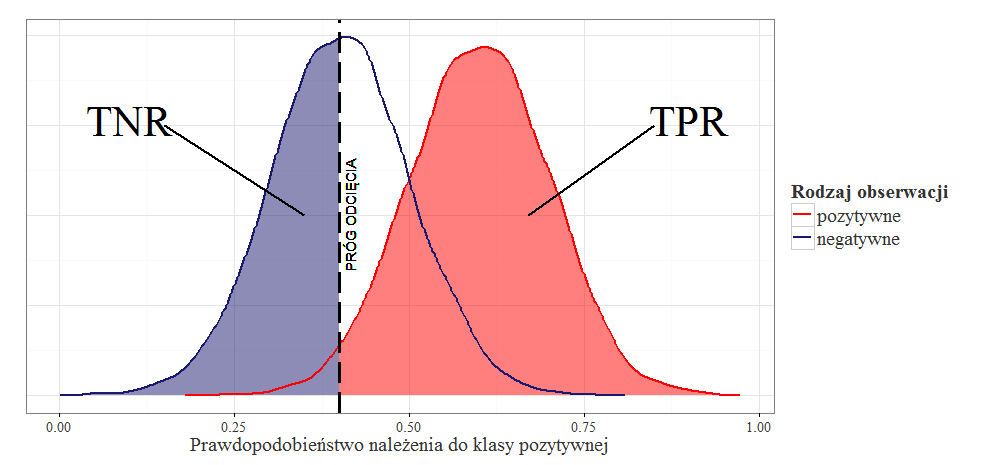
\includegraphics[width=\textwidth]{roc1.png}
    \caption{Duże TPR, ale małe TNR.}
    \label{fig:f11}
  \end{subfigure}\\
  \begin{subfigure}[h]{\textwidth}
    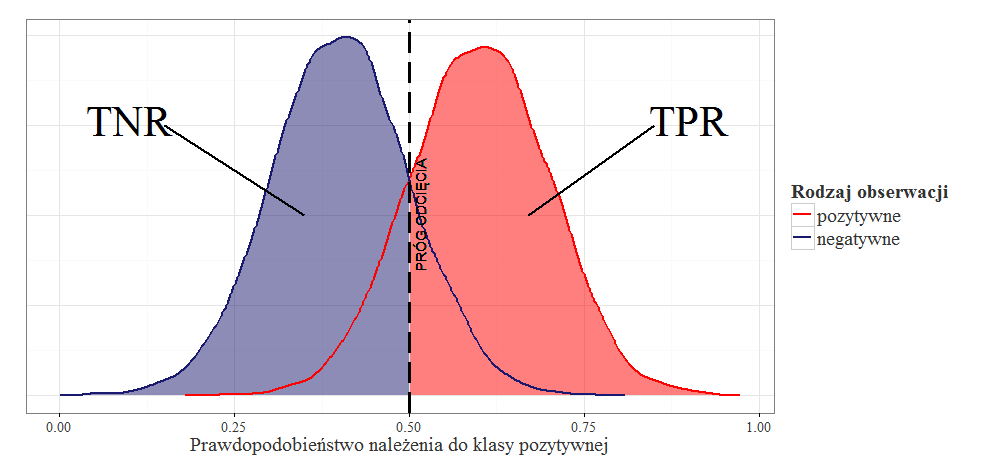
\includegraphics[width=\textwidth]{roc2.png}
    \caption{Zrównoważone TPR i TNR.}
    \label{fig:f22}
  \end{subfigure}\\
  \begin{subfigure}[h]{\textwidth}
    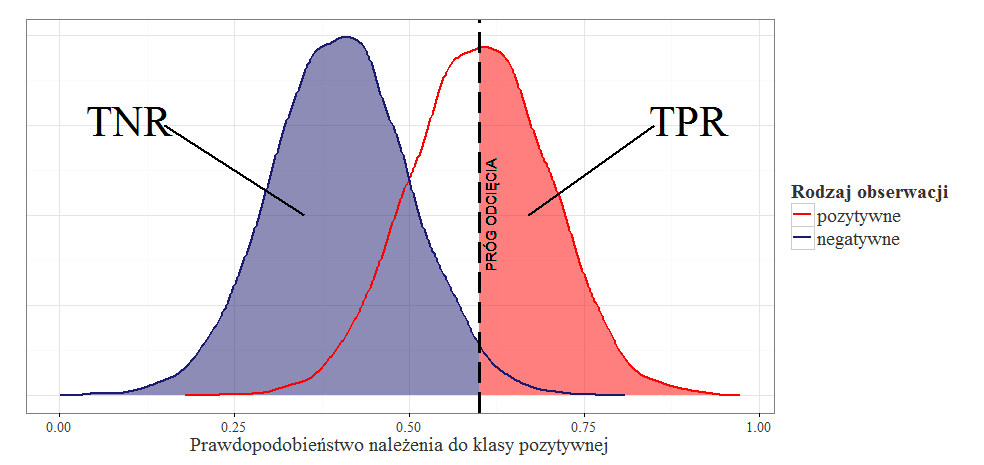
\includegraphics[width=\textwidth]{roc3.png}
    \caption{Małe TPR, ale duże TNR.}
    \label{fig:f22}
  \end{subfigure}
  \end{center}
  \caption{Sposób konstruowania krzywej ROC w przypadku dwuklasowym.}
  \label{wszystkietrzy}
\end{figure}

\vfill
\clearpage

Do stworzenia krzywej ROC, potrzebne nam będą dwa wskaźniki -- czułość (TPR, ang. \textit{True Positive Rate}) i specyficzność (TNR, ang. \textit{True Negative Rate}). Czułość definiować będziemy jako prawdopodobieństwo, że pozytywny rekord zostanie poprawnie zakwalifikowany jako pozytywny, a specyficzność jako prawdopodobieństwo, że negatywny rekord zostanie poprawnie zakwalifikowany jako negatywny. Inaczej mówiąc, czułość i specyficzność to procent poprawnie sklasyfikowanych rekordów, odpowiednio w grupie pozytywnej i negatywnej. Korzystając z tabeli jakości dopasowania (patrz Rys. \ref{tabeladopasowania}), otrzymujemy:
\begin{eqnarray*}
	TPR&=&\dfrac{TP}{TP+FN},\\
	TNR&=&\dfrac{TN}{FP+TN}.		
\end{eqnarray*}  

Ale jak stworzyć krzywą, mając tylko dwa wskaźniki? Otóż krzywa ROC to wykres punktów ($1-$TNR, TPR), wyliczonych dla różnych progów odcięcia. Czym jest zatem próg odcięcia? W większości przypadków, model generuje nam nie tylko klasę, do której powinniśmy zaklasyfikować daną obserwację, ale przede wszystkim prawdopodobieństwo, z jakim możemy coś zakwalifikować do klasy pozytywnej. Standardowo przyjmuje się, że to prawdopodobieństwo wynosi $0,5$, ale niekoniecznie musi tak być. Czasem wystarczy nam $40\%$ pewności, żeby coś zaklasyfikować jako pozytywne. Dużo tu zależy od historii, która stoi za naszymi danymi. I właśnie ten procent pewności to liczba, którą będziemy nazywać progiem odcięcia. 

\begin{figure}[h]
  \begin{subfigure}[b]{0.4\textwidth}
    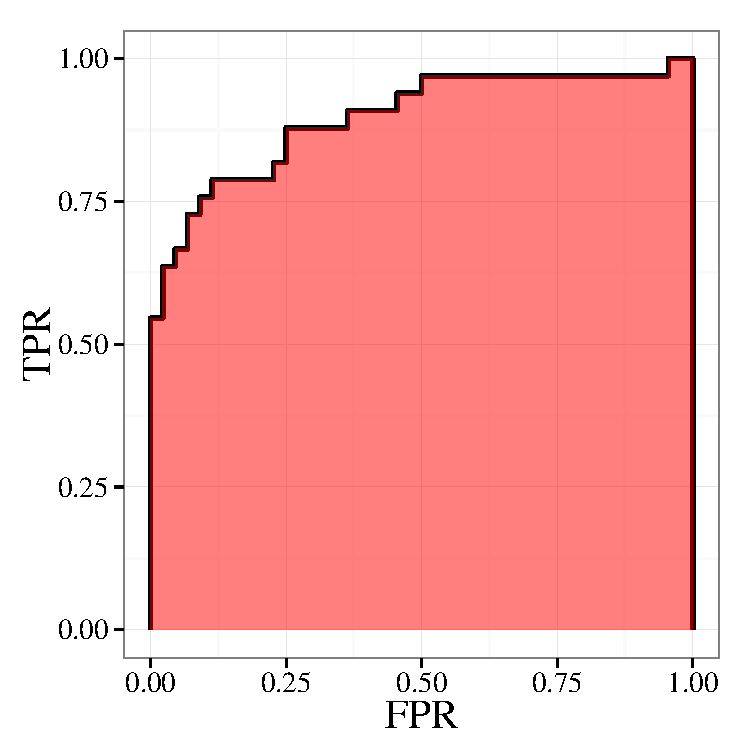
\includegraphics[width=\textwidth]{roc1.pdf}
    \caption{Standardowy sposób rysowania krzywej ROC.}
    \label{fig:f1}
  \end{subfigure}
  \hfill
  \begin{subfigure}[b]{0.4\textwidth}
    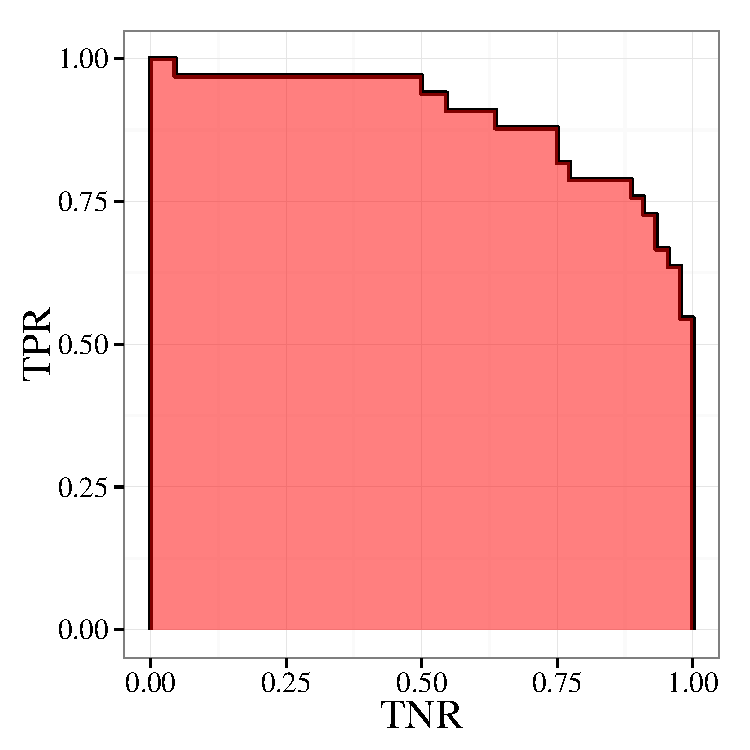
\includegraphics[width=\textwidth]{roc2.pdf}
    \caption{Krzywa ROC z TNR (zamiast FPR) na osi OX.}
    \label{fig:f2}
  \end{subfigure}
  \caption{Przykładowe krzywe ROC.}
  \label{krzyweroc}
\end{figure}

Przyjrzyjmy się rysunkowi \ref{wszystkietrzy}. Mamy tu wykresy gęstości obserwacji pozytywnych i negatywnych, w zależności od przyjętego progu odcięcia. Większość obserwacji pozytywnych osiąga około $60-$procentowe prawdopodobieństwo przynależności do klasy pozytywnej, a negatywnych $40-$procentowe prawdopodobieństwo przynależności do klasy negatywnej. Z wykresów wyraźnie widać, że poruszanie tym progiem odcięcia w prawo zwiększy nam czułość, ale zmniejszy specyficzność, natomiast poruszanie w lewo odwrotnie. Patrząc na krzywą ROC, możemy zobaczyć ich zależność od siebie na jednym wykresie i wybrać taki próg, jaki nam najbardziej odpowiada (najczęściej taki, który jest dobrym kompromisem między czułością a specyficznością). Standardowo, krzywą ROC rysuje się nie w zależności od specyficzności, tylko od $1-$specyficzności, nazywanej FPR (ang. \textit{False Positive Rate}). My jednak, by łatwiej było nam uogólnić ją na więcej wymiarów, zastosujemy tę mniej popularną reprezentację, czyli na osi OX będziemy przedstawiać specyficzność (patrz Rys.\ref{krzyweroc}). 

Idealna krzywa to taka, która ma duże TPR i małe FPR, tworzy zatem kwadrat jednostkowy. Zła krzywa, czyli taka, która powstaje, gdy model daje losowe wyniki, to taka, która jest przekątną tego kwadratu. Ponieważ, patrząc na dwie często wielokrotnie przecinające się krzywe ROC, odpowiadające różnym modelom, ciężko jest stwierdzić, która krzywa jest lepsza, wprowadzono współczynnik AUC, czyli pole pod tą krzywą, który pozwala łatwiej to ocenić. Idealny model ma współczynnik AUC równy $1$, a model losowy charakteryzuje się AUC równym $0,5$. Na rysunku \ref{krzyweroc} łatwo widać, że w naszym przypadku (czyli z inaczej zdefiniowaną osią OX) współczynnik AUC definiuje się identycznie.       

\section{Krzywa ROC w przypadku regresji porządkowej}

\begin{figure}[h]
	\begin{center}
  \begin{subfigure}[h]{\textwidth}
    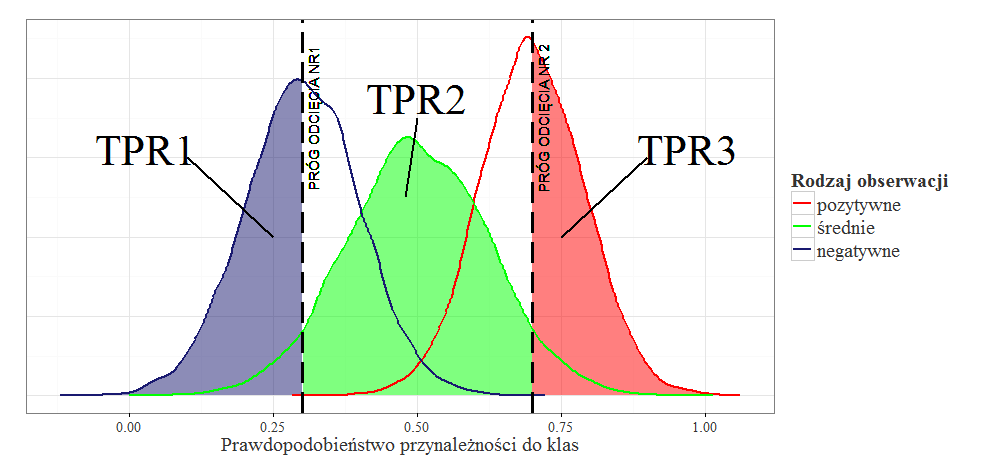
\includegraphics[width=\textwidth]{roc_trzy1.png}
  \end{subfigure}\\
  \begin{subfigure}[h]{\textwidth}
    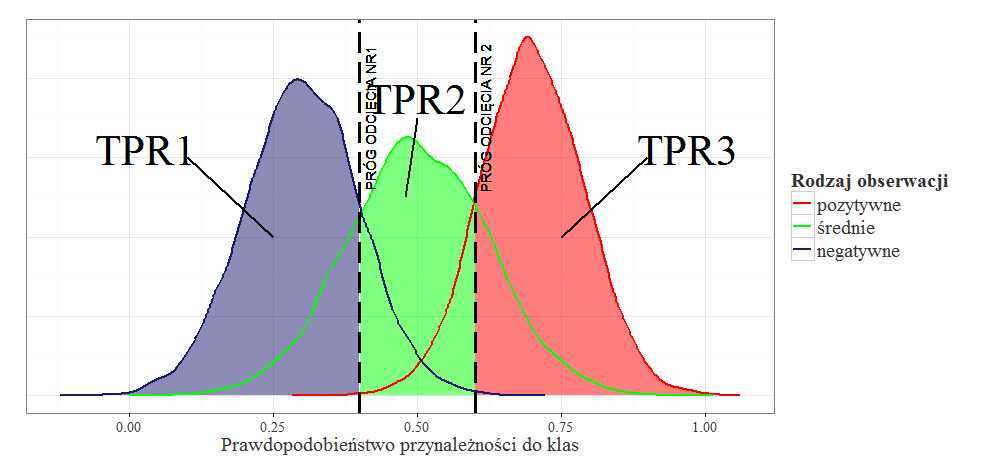
\includegraphics[width=\textwidth]{roc_trzy2.png}
  \end{subfigure}
  \end{center}
  \caption{Sposób konstruowania krzywej ROC w przypadku trzyklasowym.}
  \label{trzyklasowy}
\end{figure}

W przypadku regresji porządkowej nie będzie już tak łatwo. Przede wszystkim nie mamy tu podziału na klasę pozytywną i negatywną, jak więc stworzyć współczynnik FPR? Można próbować robić to parami tzn. traktować jedną z klas jako pozytywną, a pozostałe połączyć w jedną i traktować jako negatywną. Robiąc w ten sposób z każdą klasą, otrzymamy $r$ (bo tyle jest możliwych poziomów zmiennej odpowiedzi) krzywych ROC, a tym samym $r$ współczynników AUC. Jako ostateczne AUC przyjmuje się wtedy średnią z nich. Nie jest to jednak dobry wskaźnik. Może się bowiem zdarzyć tak, że współczynnik między środkowymi klasami wyjdzie duży, natomiast ten między klasami skrajnymi słaby, tworząc tym samym nienajgorszą średnią. Nie jest to dobre, gdyż często zależy nam na dobrym odróżnieniu właśnie klas skrajnych. Wyobraźmy sobie, że chcemy sprawdzić, czy komuś spodobałaby się sprzedawana przez nas książka. Możliwe odpowiedzi to: bardzo mi się podoba, podoba mi się, nie mam zdania, nie podoba mi się, bardzo mi się nie podoba. Jasne jest, że wolelibyśmy oddzielić klientów, którym bardzo spodobałaby się książka od tych, którym bardzo by się nie spodobała, a nie na przykład tych, którym by się nie spodobała od tych, którym by się bardzo nie spodobała. Żeby udało nam się poradzić sobie z takim problemem, trzeba spojrzeć na niego globalnie.   

Opisując krzywą ROC w przypadku dwuklasowym powiedzieliśmy sobie, że będziemy rozważać nie zależność TPR od FPR, ale TPR od TNR. Dlaczego? Właśnie po to, żebyśmy teraz mogli ją łatwiej uogólnić. Zarówno TPR, jak i TNR jest to procent poprawnie sklasyfikowanych odpowiednio pozytywnych bądź negatywnych obserwacji. Nic nie staje zatem na przeszkodzie, by stworzyć $r$ takich współczynników ($\text{TPR}1, \ldots, \text{TPR}r$), każdy odpowiadający procentowi poprawnie sklasyfikowanych obserwacji z $i-$tej klasy. Przyjmując różne progi odcięcia (patrz Rys. \ref{trzyklasowy}), których tym razem będzie $r-1$, możemy narysować krzywą ROC, a raczej pewną hiperpowierzchnię. Oczywiście jest to możliwe tylko w przypadku trzyklasowym (patrz Rys. \ref{3d}), ale rysunek taki i tak jest raczej mało czytelny. 

\begin{figure}[h]
\begin{center}
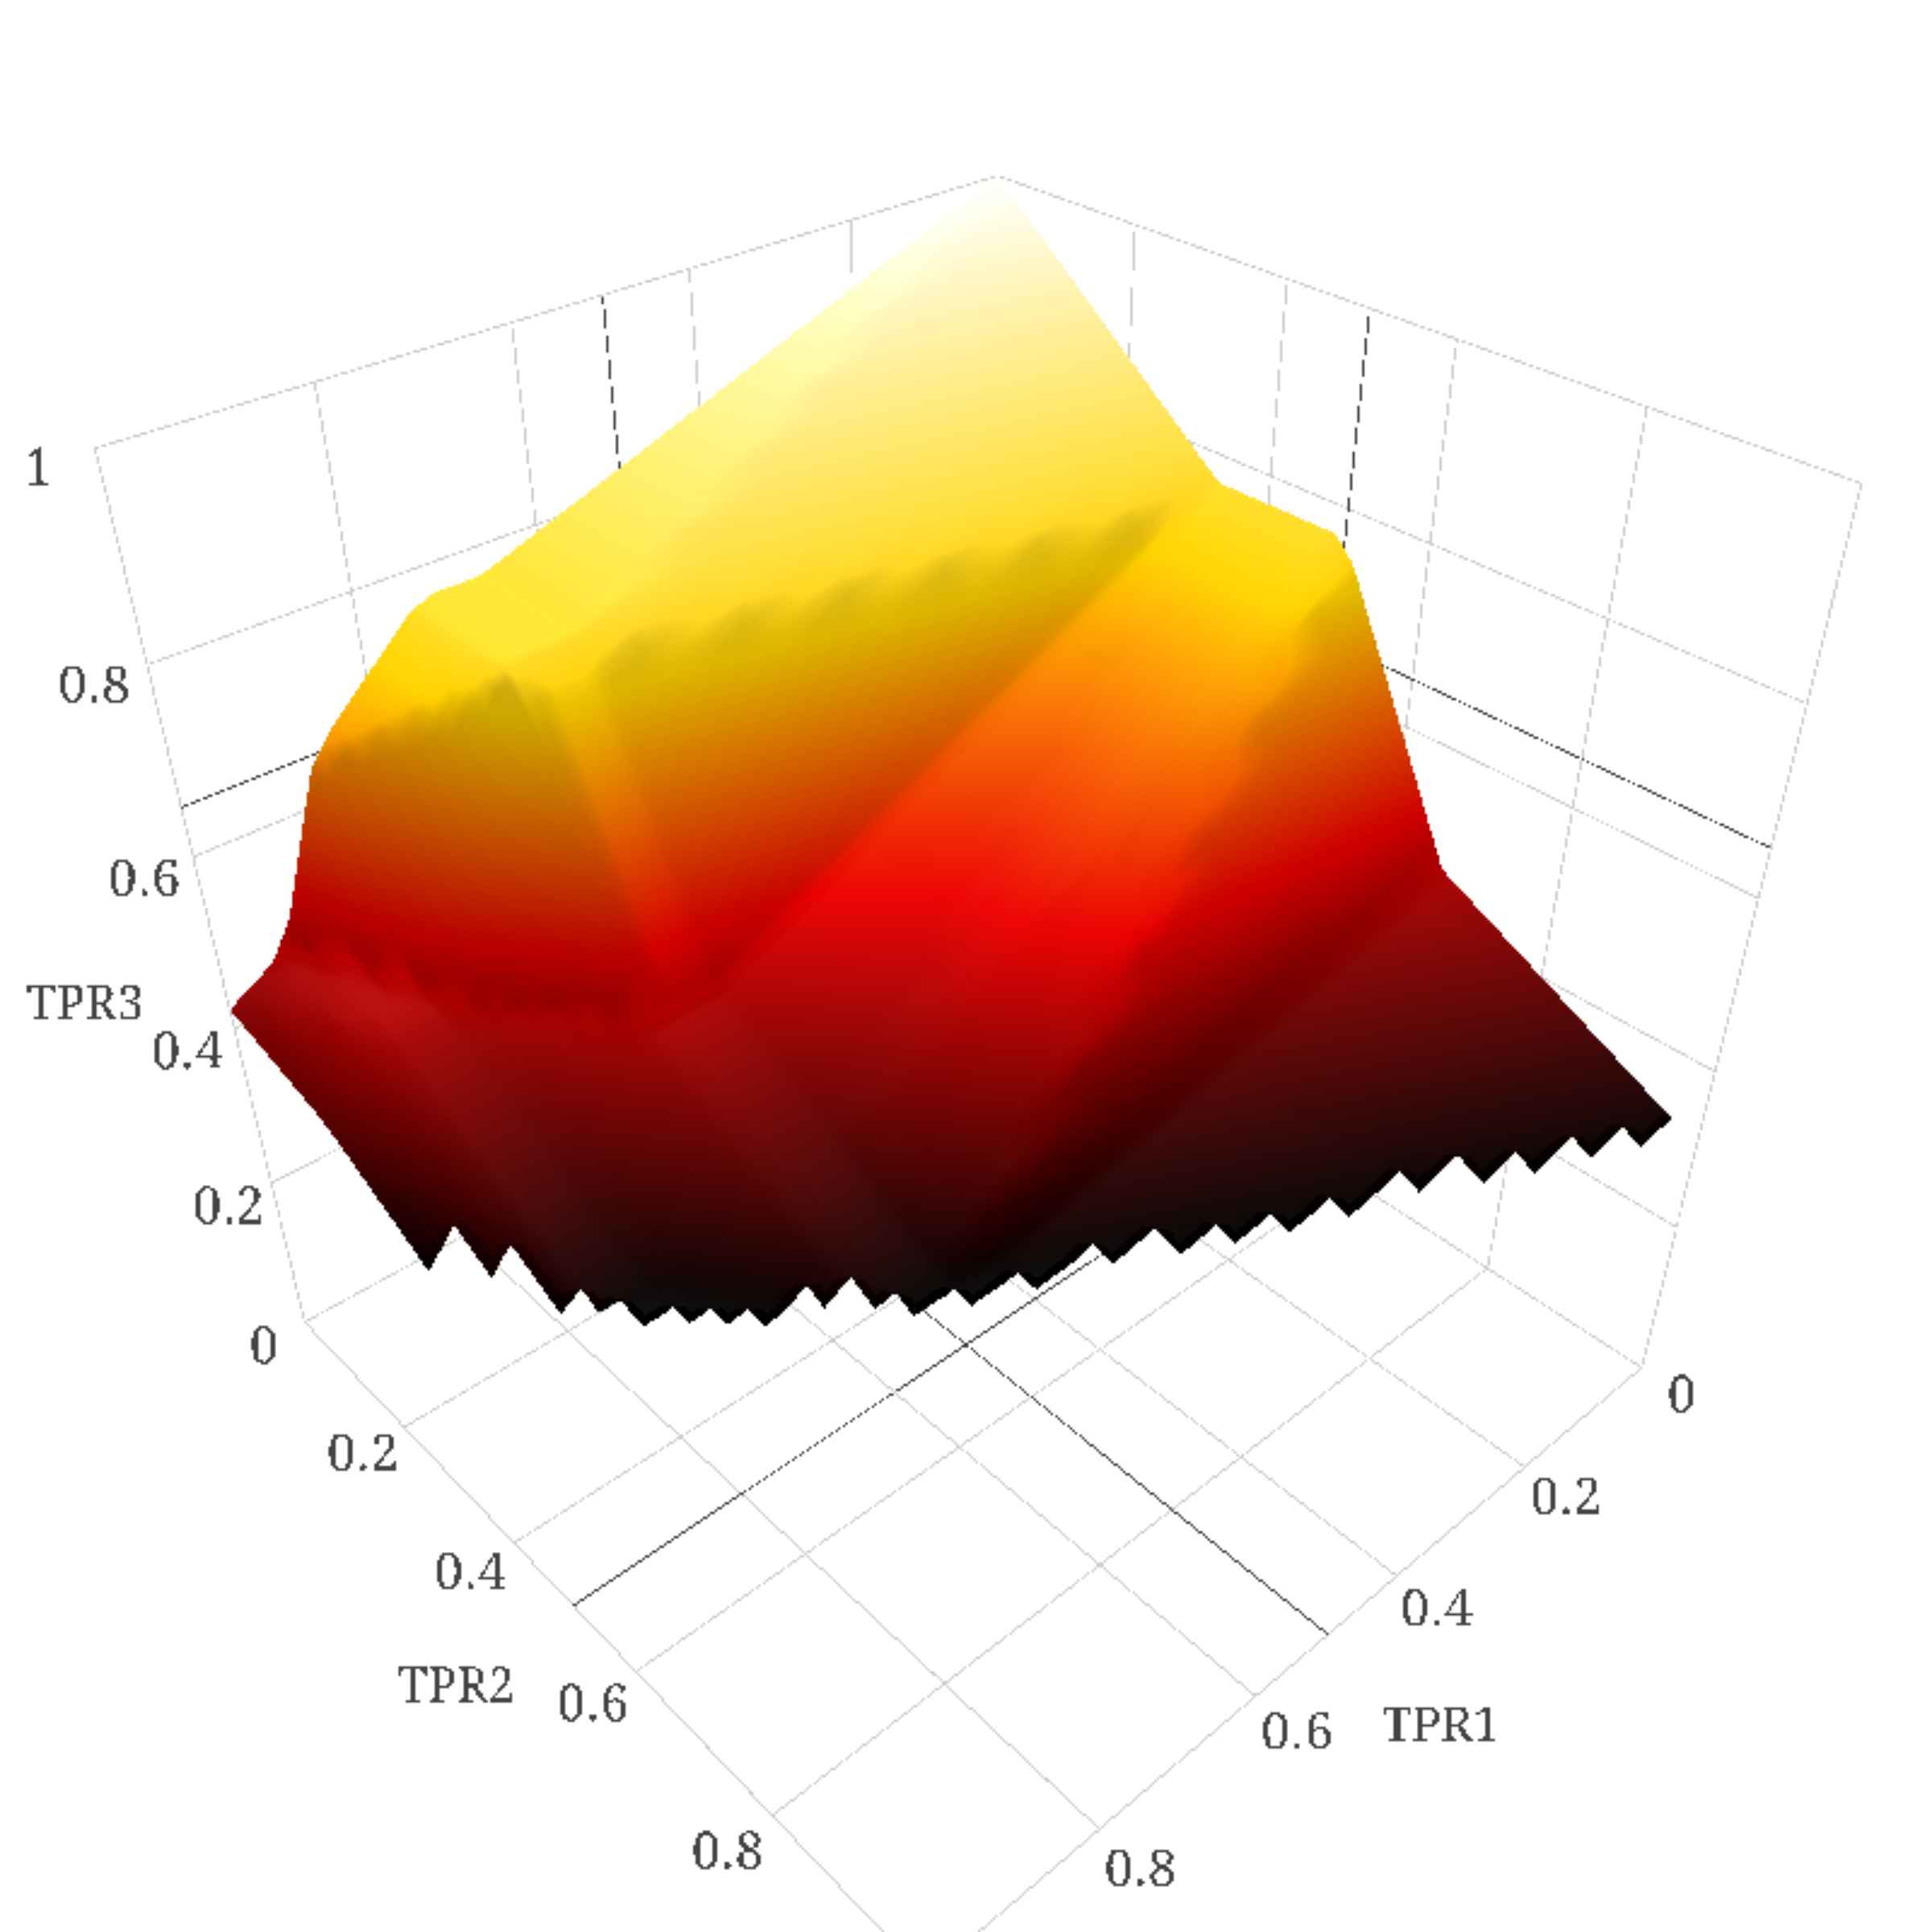
\includegraphics[scale=0.5]{roc3d.png}
\end{center}
\caption{Krzywa ROC w przypadku trzyklasowym.}
\label{3d}
\end{figure}

\section{Współczynnik VUS}

Po co zatem tworzyć wielowymiarową krzywą ROC, skoro i tak trudno cokolwiek z niej odczytać? Otóż głównie po to, by otrzymać współczynnik AUC, który, będąc konkretną liczbą, jest znacznie prostszy w interpretacji. W przypadku więcej niż dwuwymiarowym będziemy go nazywać VUS (ang. \textit{Volume Under the Surface}). 

Jako, że liczenie objętości pod hiperpłaszczyzną jest numerycznie raczej trudnym zadaniem, w celu wyliczenia współczynnika VUS, skorzystamy z jego nieco innej interpretacji niż tylko pole pod krzywą ROC. Wróćmy znów do przypadku dwuklasowego i przyjrzyjmy się wykresowi \ref{fig:f2}. Na osi OY mamy współczynnik TNR, czyli prawdopodobieństwo, że wyestymujemy klasę negatywną pod warunkiem, że klasa rzeczywiście jest negatywna. Równoważnie, można to zapisać jako prawdopodobieństwo, że prawdopodobieństwo odpowiadające negatywnej obserwacji jest mniejsze niż pewien próg odcięcia. Analogicznie TPR to prawdopodobieństwo, że prawdopodobieństwo odpowiadające pozytywnej obserwacji jest większe niż próg odcięcia. Łącząc oba wyniki otrzymamy, że współczynnik AUC to nic innego tylko prawdopodobieństwo, że losowo wybrana pozytywna obserwacja będzie mieć wyższe prawdopodobieństwo niż losowo wybrana negatywna obserwacja. Innymi słowy, będą one dobrze uporządkowane. Łatwo to już uogólnić na więcej, w naturalny sposób uporządkowanych, wymiarów. Interesować nas będzie pewna estymacja tego prawdopodobieństwa. Łatwo można zauważyć, że będzie nią tzw. statystyka $U$  Manna–Whitney'a–Wilcoxona (por. \cite{roc1}, \cite{roc2}), czyli wyrażenie:

$$
VUS = \dfrac{1}{n_1n_2\cdot\ldots\cdot n_r}\sum_{i_1=1}^{n_1}\sum_{i_2=1}^{n_2}\ldots\sum_{i_r=1}^{n_r}\mathbb{I}_{\lbrace f(\mathbf{x}_{i_1}^1)<\ldots<f(\mathbf{x}_{i_r}^r)\rbrace},
$$
gdzie $\textbf{x}_i^j$ oznacza $i-$ty wektor cech $\mathbf{x}$ o prawdziwej klasie $j$, $n_i$ to liczba obserwacji zaklasyfikowanych przez nas jako klasa $i$, a $f$ to pewna funkcja, która zwraca liczbę rzeczywistą, mającą estymować uporządkowanie obserwacji. 

Krzywa ROC i współczynnik VUS jest więc dość prostym, bardzo łatwo interpretowalnym i pomocnym narzędziem do oceny jakości modelu i podejmowania decyzji, który model jest najlepszy. Największą jego wadą wydaje się konieczność znania prawdopodobieństw przynależności do klas (lub po prostu funkcji, która pozwoli nasze obserwacje uporządkować), a nie każda metoda takie prawdopodobieństwa zwraca (np. nie robią tego sieci neuronowe). Trzeba wtedy odwołać się do prostszych metod (takich jak procent poprawności dopasowania lub czułość). Większość modeli oferuje jednak taką możliwość, więc niewątpliwie warto z tego narzędzia diagnostycznego korzystać.


%%%%%%%%%%%%%%%%%%%%%%%%%%%%%%%%%%%%%%%%%%%%%%%%%%%%%%%%%%%%%%%%%%%%%%%%%%%%%%%%%%%%%%%%%%%%%%%%%%%%%%%%%%%%%%%%%%%%%%%%%%%%%

\appendix

\chapter{fdaaggfdadfsd}

%-----------------------------------------------------------------------------%

\begin{thebibliography}{9}
	\bibitem{fh} Frank E., Hall M., A simple approach to ordinal classification, \emph{Proceedings of the European Conference on Machine Learning}, Freibourg, Niemcy, 2001, str. 146--156.
	\bibitem{nna} Cheng J., Wang Z., Pollastri G., A neural network approach to ordinal regression, \emph{Neutral Networks}, Hong Kong, 2008.
	\bibitem{pom} Dobson A. J., An Introduction to Generalized Linear Models, 2nd Edition, 2001 
	\bibitem{svm} Chu W., Sathiya Keerthi S., \emph{Support Vector Ordinal Regression}
	\bibitem{reg} Chu W., Ghahramani Z., \emph{Gaussian Processes for Ordinal Regression}
	\bibitem{reg2} Ebden M., \emph{Gaussian Processes for Classification: A Quick Introduction}, August 2008.
	\bibitem{reg3} Ebden M., \emph{Gaussian Processes for Regression: A Quick Introduction}, August 2008.
	\bibitem{reg4} Rasmussen C., Williams C., \emph{Gaussian Processes for Machine Learning}, 2006.
	\bibitem{roc1} Waegman W., De Baets B., A survey on ROC-based ordinal regression, w: Fürnkranz J., Hüllermeier E. (Eds.), \emph{Preference Learning}, Springer, 2010, str. 127-154.
	\bibitem{roc2} Nakas C.T., Yiannoutsos C.T., Ordered Multiple Class Receiver Operating Characteristic (ROC) Analysis, \emph{Encyclopedia of Biopharmaceutical Statistics}, Taylor and Francis, 2006.
\end{thebibliography}

%-----------------------------------------------------------------------------%

\makestatement
\end{document}
